\section{System Under Test}
\label{sec:system:sut}
% Explain SUT
% Components of Interest
% Purely Functional Components
% Present SUT

To design a benchmarking instrument that evaluates \gls{sm} systems, we first have to define the system and the components that are included in the benchmark. The components relevant to the benchmark are described in the \gls{sut}. However, even though the benchmark has to deal with numerous components related to the \gls{sm} system ant its surrounding environment, not all are relevant to measure to satisfy the benchmarking objectives.

Therefore, we split the components of the \gls{sut} in two categories according to the practices outlined by Folkerts et al. \cite{folkerts2012benchmarking}. The first group of components are labelled \textit{Components of Interest}. These components are of principal interest to the benchmark and have to be measured. The second group of components is labelled as \textit{Purely Functional Components}. The components in the latter group are present in the \gls{sut} in order for the benchmarking instrument to work correctly. However, measuring these components is not of importance relating to the objectives of the benchmark.

In \cref{fig:sut} we present the \gls{sut} for the benchmarking instrument. In the following sections, we elaborate on the  \textit{Components of Interest} (\cref{sec:system:sut:components-interest}) and \textit{Purely Functional Components} (\cref{sec:system:sut:components-functional})  present in this system.

\begin{figure}[!t]
    \centering
    
    \scalebox{.8}{    
    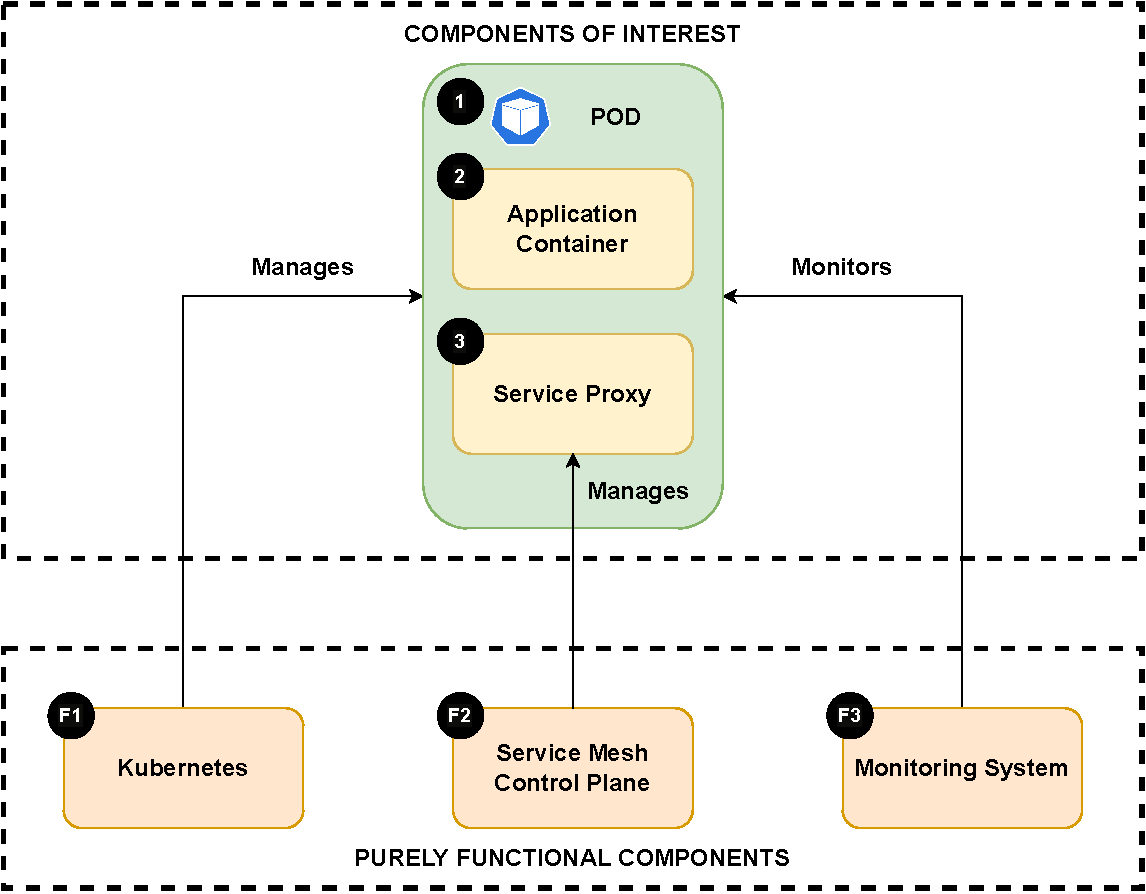
\includegraphics[width=\linewidth]{4_system_design/figures/system-under-test.pdf}
    }
    
    \caption{The \gls{sut} for benchmarking \gls{sm} systems.}
    
    \label{fig:sut}
\end{figure}

\subsection{Components of Interest}
\label{sec:system:sut:components-interest}
% Elaborate on the components of interest
% Data Path of Traffic
% Pod containing the service
% - Application Pod
% - Service Mesh Proxy (data plane)

The \textit{Components of Interest} are aligned with the objectives as presented in \cref{sec:system:objectives}. In the context of a \gls{sm} system, we aim to measure and evaluate the components present in the data path of a software service. Therefore, in the context of a \gls{k8s} cluster running a \gls{sm}, we evaluate the performance of software services that live in the \gls{k8s} specific abstraction, the \gls{pod} \designref{1}.

To measure the service and the service traffic, we measure the application container \designref{2} and the data plane components of a \gls{sm} \designref{3}.

\subsection{Purely Functional Components}
\label{sec:system:sut:components-functional}
% Elaborate on the functional components
% Metric Services - Prom
% Control Plane components of sm
% - More detail?

To be able to run the benchmark, we require the several components. First, we run the benchmark on a \gls{k8s} cluster \designref{F1}. Furthermore, a \gls{sm} system introduces several control plane components, which are required for the service mesh to correctly function \designref{F2}. However, since our objectives are to measure the data path of a \gls{sm} they are not of importance to the benchmarking instrument. Additionally, we introduce a metric collector and monitoring system in the cluster \designref{F3}, which will be used to collect and time series data of the pods and containers residing in the \gls{k8s} cluster.